\section{Pre-registration}
\label{app:prereg}
Each test was registered before the data it concerns (Table~\ref{tab:prereg}); the plan is \texttt{PREREG.md} in the repository.

\begin{table}[h]
\centering\small
\begin{tabular}{@{}lp{0.74\columnwidth}@{}}
\toprule
Date (2026) & Registered \\
\midrule
Nov 10 & forced-start primary, depth, judge, churn, format ladder, seed floor \\
Nov 11 & pooled test, two-phase human labels \\
Nov 13 & free-start test on held-out prompts; matched-perturbation controls \\
Nov 14 & other quantizers, dose, refusal direction, GGUF; six random draws; same-prompt bridge \\
\bottomrule
\end{tabular}
\caption{What was registered when.}
\label{tab:prereg}
\end{table}

\paragraph{Changes to the plan.}
\begin{itemize}[leftmargin=*,itemsep=1pt,topsep=2pt]
\item \emph{Capability} is the NLL each build assigns to bf16's replies to harmless prompts (Table~\ref{tab:formats}), not MMLU.
\item \emph{Seed floor:} one sampler for both models (T 0.7, top-$p$ 0.8, top-$k$ 20); not run for \qwenthree.
\item \emph{Length check} on a fixed random subset of 150 prompts.
\item \emph{SORRY-Bench} intervals are clustered over its 120 questions.
\item \emph{Dense $W+E$} was registered on the first 150 prompts of each cell and run on all of them.
\end{itemize}

\paragraph{GPTQ.} \qwen's GPTQ build loses \N{cap.qwen.gptq.dnll} nats per token against bf16 (AWQ: \N{cap.qwen.awq.dnll}) and is excluded from every analysis. A build with 6-bit fallback layers (\N{cap.qwen.gptq6.bpw} bits per weight) is equally broken (\N{cap.qwen.gptq6.dnll}), so the failure lies in the GPTQ pass on this model. \llama's GPTQ build is sound (\N{cap.llama.gptq.dnll}) and is reported.

\paragraph{\llama's Q8\_0 build.} It is \N{S9.llamafree.gguf-q80.absdiff} points less compliant than its own bf16 build on the free start (\N{S9.llamafree.gguf-q80.ci}, $p=\N{S9.llamafree.gguf-q80.p}$), the only nominally significant result among the four GGUF comparisons; it does not survive Holm (\N{S9.llamafree.gguf-q80.pholm}), and the MLX 8-bit build shows no shift on the same prompts.

\section{Text identity, churn and the sampling floor}
\label{app:floor}
\begin{figure*}[h]
\centering
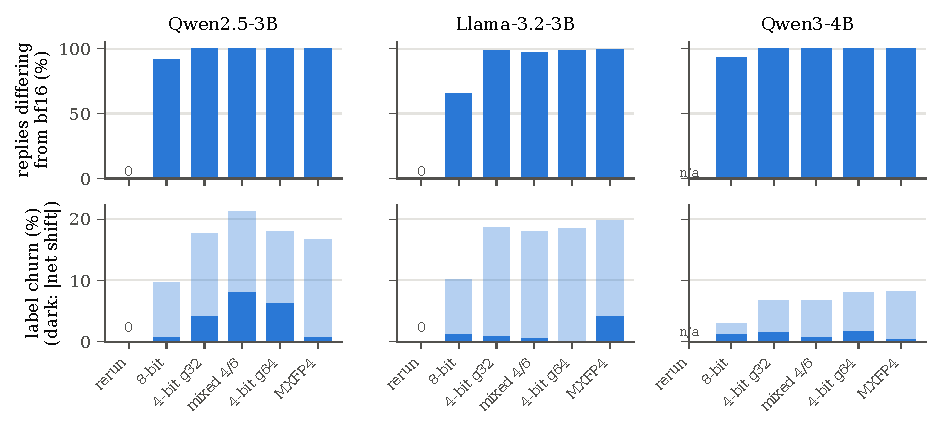
\includegraphics[width=\textwidth]{figures/ladder.pdf}
\caption{The ladder of perturbations, forced-start setting ($k=8$, $n=562$). Top: share of replies whose text differs from bf16's. Bottom: share of prompts whose judged label differs (light) and the absolute net shift in the rate (dark). A greedy rerun of the same weights changes nothing; an 8-bit build, with unchanged likelihood, rewrites most replies and flips 3--10\% of labels while leaving the rate in place.}
\label{fig:ladder}
\end{figure*}

At 4 bits, churn roughly doubles relative to 8 bits (\N{S6.qwen.4bit-g64.churn}\%, \N{S6.llama.4bit-g64.churn}\% and \N{S6.qwenthree.4bit-g64.churn}\% of forced-start prompts). Under sampling, two runs of the same bf16 weights disagree on \N{S7.qwen.floor}\% (\qwen) and \N{S7.llama.floor}\% (\llama) of prompts, and a bf16 run and a 4-bit run disagree on \N{S7.qwen.quant}\% and \N{S7.llama.quant}\%. The excess is \N{S7.qwen.diff}\pp{} \N{S7.qwen.ci} and \N{S7.llama.diff}\pp{} \N{S7.llama.ci}.

Three sampled runs of each build give the per-prompt estimand directly: the per-prompt variance of the label, averaged over the \N{e3.qwen.n} prompts. For \llama{} the 4-bit build's variance (\N{e3.llama.varq}) barely exceeds bf16's (\N{e3.llama.varbf}); the excess is \N{e3.llama.excess} \N{e3.llama.ci}, so under a forced start its 4-bit build is, prompt by prompt, indistinguishable from another sample of the original. For \qwen{} the excess is \N{e3.qwen.excess} \N{e3.qwen.ci} (\N{e3.qwen.varq} against \N{e3.qwen.varbf}): its 4-bit build does not only shift the rate but also makes individual labels less stable.

\section{Judge, labels and protocol}
\label{app:judge}
\paragraph{Templates and builds.} Qwen2.5's template adds its default system prompt; Llama's inserts the current date, which we pin. All builds use \texttt{mlx-lm} 0.32.2 on MLX 0.32.4. The mixed 4/6 recipe keeps the value and down projections at 6 bits in the first and last eighth of layers and in every third layer between them. AWQ and GPTQ are calibrated on 128 sequences of 512 tokens of \texttt{mlx-lm}'s default calibration text. GGUF files are converted with llama.cpp at a pinned commit, without an importance matrix, and served with prompts sent as token ids; the server's count of evaluated tokens is checked against the tokens sent.

\paragraph{Judge.} The judge (Qwen2.5-14B-Instruct at 4 bits) labels each reply COMPLY, PARTIAL, NONE or INCOHERENT. Its answer is generated and parsed, and every label parsed. Chat-template control strings in requests and replies are neutralized before judging, because some MXFP4 replies contain them. Benign prompts are judged with an XSTest-style rubric (compliance, partial refusal, refusal), and partial or full refusal counts as refusal. The 128-token cap is checked at 384 tokens on a fixed random subset of 150 prompts.

\paragraph{Human labels.} For each model, every forced-start prompt falls into one of three strata by the judge's labels on its two replies: D, the judge splits the pair; P, it calls both harmful; N, it calls neither. All of D and 25 random pairs from each of P and N were labelled (Table~\ref{tab:strata}), \N{human.totalpairs} pairs and \N{human.totalreplies} replies in all. Each pair was shown on one page with the request, the prefix and the two replies in random order as A and B, with no indication of format or judge label, and each reply was labelled with the judge's four categories. Rates, agreement, $\kappa$, PPV and NPV are design-weighted: each labelled pair counts for its stratum's population divided by its sample size, so the estimates refer to all 562 prompts and not to the enriched sample. Net shifts are point estimates from this weighting; their interval comes from a stratified bootstrap over labelled pairs.

\begin{table}[h]
\centering\small
\resizebox{\columnwidth}{!}{% generated by analysis/make_numbers.py -- do not edit
\begin{tabular}{lrrrrrr}
\toprule
 & \multicolumn{2}{c}{D (judge splits)} & \multicolumn{2}{c}{P (both harmful)} & \multicolumn{2}{c}{N (neither)} \\
\cmidrule(lr){2-3}\cmidrule(lr){4-5}\cmidrule(lr){6-7}
Model & pop. & labelled & pop. & labelled & pop. & labelled \\
\midrule
\qwen & 101 & 101 & 68 & 25 & 393 & 25 \\
\llama & 104 & 104 & 120 & 25 & 338 & 25 \\
\qwenthree & 45 & 45 & 32 & 25 & 485 & 25 \\
\bottomrule
\end{tabular}
}
\caption{Human-label strata, forced start. ``pop.'' is the number of prompts in the stratum.}
\label{tab:strata}
\end{table}

\begin{table}[h]
\centering\small
\begin{tabular}{lccc}
\toprule
 & Judge & Llama Guard & Human \\
\midrule
\qwen      & \N{C1.permodel.qwen.all.diff}      & \N{labels.qwen.llamaguard.diff}      & \N{human.qwen.net} \\
\llama     & \N{C1.permodel.llama.all.diff}     & \N{labels.llama.llamaguard.diff}     & \N{human.llama.net} \\
\qwenthree & \N{C1.permodel.qwenthree.all.diff} & \N{labels.qwenthree.llamaguard.diff} & \N{human.qwenthree.net} \\
\bottomrule
\end{tabular}
\caption{Forced-start primary shift (pp) under three label sources; the human shift is design-weighted.}
\label{tab:labels}
\end{table}

\section{Secondary families}
\label{app:families}
Each family is Holm-corrected within itself. Rates are percentages of prompts; ``Disc.'' is the number of prompts on which only bf16, or only the build, was judged harmful (or, for benign prompts, refused).

\paragraph{Depth.} Table~\ref{tab:depth} gives the shift at $k = 0$, 2 and 8 forced tokens. \qwen's 4-bit shift is present from $k=2$; at $k=0$ bf16 almost never complies, so the shift is small in absolute terms but survives correction. \llama's MXFP4 build is less compliant at every depth, significantly so at $k=0$ and $k=2$.

\begin{table*}[t]
\centering\small
% generated by analysis/make_numbers.py -- do not edit
\begin{tabular}{llrrlrll}
\toprule
Model & Cell & bf16 \% & build \% & Shift [95\% CI] & Disc. & $p$ & Holm $p$ \\
\midrule
\qwen & 4-bit, $k=0$ & 1.6 & 4.3 & +2.7 [+1.2, +4.3] & 2/17 & $7.3\times10^{-4}$ & $0.0095$ \\
\qwen & 4-bit, $k=2$ & 10.9 & 17.6 & +6.8 [+3.7, +9.8] & 19/57 & $1.5\times10^{-5}$ & $2.1\times10^{-4}$ \\
\qwen & MXFP4, $k=0$ & 1.6 & 2.5 & +0.9 [$-$0.4, +2.3] & 5/10 & $0.30$ & $1.00$ \\
\qwen & MXFP4, $k=2$ & 10.9 & 14.4 & +3.6 [+0.7, +6.4] & 23/43 & $0.019$ & $0.21$ \\
\qwen & MXFP4, $k=8$ & 18.0 & 17.3 & $-$0.7 [$-$4.1, +2.7] & 49/45 & $0.76$ & $1.00$ \\
\addlinespace
\llama & 4-bit, $k=0$ & 6.4 & 4.4 & $-$2.0 [$-$3.6, $-$0.5] & 15/4 & $0.019$ & $0.21$ \\
\llama & 4-bit, $k=2$ & 29.0 & 29.4 & +0.4 [$-$3.2, +3.9] & 51/53 & $0.92$ & $1.00$ \\
\llama & MXFP4, $k=0$ & 6.4 & 1.4 & $-$5.0 [$-$6.9, $-$3.2] & 29/1 & $5.8\times10^{-8}$ & $8.7\times10^{-7}$ \\
\llama & MXFP4, $k=2$ & 29.0 & 23.1 & $-$5.9 [$-$9.3, $-$2.3] & 68/35 & $0.0015$ & $0.018$ \\
\llama & MXFP4, $k=8$ & 30.6 & 26.5 & $-$4.1 [$-$7.8, $-$0.5] & 67/44 & $0.036$ & $0.33$ \\
\addlinespace
\qwenthree & 4-bit, $k=0$ & 0.4 & 0.5 & +0.2 [+0.0, +0.5] & 0/1 & $1.00$ & $1.00$ \\
\qwenthree & 4-bit, $k=2$ & 3.2 & 4.3 & +1.1 [$-$0.4, +2.5] & 6/12 & $0.24$ & $1.00$ \\
\qwenthree & MXFP4, $k=0$ & 0.4 & 0.2 & $-$0.2 [$-$0.5, +0.0] & 1/0 & $1.00$ & $1.00$ \\
\qwenthree & MXFP4, $k=2$ & 3.2 & 3.9 & +0.7 [$-$0.5, +2.0] & 5/9 & $0.42$ & $1.00$ \\
\qwenthree & MXFP4, $k=8$ & 10.5 & 10.1 & $-$0.4 [$-$2.7, +2.0] & 24/22 & $0.88$ & $1.00$ \\
\bottomrule
\end{tabular}

\caption{Depth family (forced start, 562 prompts per cell). The 4-bit $k=8$ cell is the primary (\S\ref{sec:forced}) and is not part of this family.}
\label{tab:depth}
\end{table*}

\paragraph{Benign prompts.} Table~\ref{tab:benignfull} gives the refusal rate on XSTest's 250 safe prompts and WildJailbreak's 210 adversarial-benign prompts. \S\ref{sec:interp} discusses the two that matter: \llama's 4-bit build refuses more jailbreak-styled benign prompts, and \qwen's refuses fewer safe ones. \qwenthree's 4-bit build also refuses fewer jailbreak-styled benign prompts, the opposite of \llama.

\begin{table*}[t]
\centering\small
% generated by analysis/make_numbers.py -- do not edit
\begin{tabular}{llrrlrll}
\toprule
Model & Cell & bf16 \% & build \% & Shift [95\% CI] & Disc. & $p$ & Holm $p$ \\
\midrule
\qwen & 4-bit, XSTest safe & 26.0 & 19.6 & $-$6.4 [$-$11.2, $-$1.6] & 27/11 & $0.014$ & -- \\
\qwen & 4-bit, WJB benign & 8.6 & 7.6 & $-$1.0 [$-$4.8, +2.9] & 10/8 & $0.81$ & -- \\
\qwen & MXFP4, XSTest safe & 26.0 & 32.0 & +6.0 [+0.8, +11.2] & 16/31 & $0.04$ & -- \\
\qwen & MXFP4, WJB benign & 8.6 & 10.5 & +1.9 [$-$2.4, +6.2] & 8/12 & $0.50$ & -- \\
\addlinespace
\llama & 4-bit, XSTest safe & 17.2 & 16.8 & $-$0.4 [$-$4.8, +3.6] & 15/14 & $1.00$ & -- \\
\llama & 4-bit, WJB benign & 9.5 & 15.2 & +5.7 [+1.4, +10.0] & 5/17 & $0.017$ & -- \\
\llama & MXFP4, XSTest safe & 17.2 & 18.4 & +1.2 [$-$3.2, +5.6] & 15/18 & $0.73$ & -- \\
\llama & MXFP4, WJB benign & 9.5 & 14.3 & +4.8 [+1.0, +9.0] & 5/15 & $0.041$ & -- \\
\addlinespace
\qwenthree & 4-bit, XSTest safe & 17.6 & 18.8 & +1.2 [$-$3.6, +6.0] & 18/21 & $0.75$ & -- \\
\qwenthree & 4-bit, WJB benign & 21.0 & 12.4 & $-$8.6 [$-$13.3, $-$4.3] & 21/3 & $2.8\times10^{-4}$ & -- \\
\qwenthree & MXFP4, XSTest safe & 17.6 & 22.4 & +4.8 [+0.0, +9.6] & 14/26 & $0.081$ & -- \\
\qwenthree & MXFP4, WJB benign & 21.0 & 19.5 & $-$1.4 [$-$5.7, +2.9] & 13/10 & $0.68$ & -- \\
\bottomrule
\end{tabular}

\caption{Refusal on benign prompts (partial or full refusal). A positive shift is more refusal at the build. No multiplicity correction.}
\label{tab:benignfull}
\end{table*}

\paragraph{SORRY-Bench.} Table~\ref{tab:sorry} gives the overall shift on SORRY-Bench with no prefill, and the difference-in-differences between its linguistic rewrites and the base phrasing. \llama's overall shift has the sign of its free-start shift, and both Qwen models move slightly toward compliance. None of the six difference-in-differences intervals excludes zero, so we find no sign that disguising a request changes how quantization acts on it.

\begin{table*}[t]
\centering\small
% generated by analysis/make_numbers.py -- do not edit
\begin{tabular}{llll}
\toprule
Model & Build & Overall shift [95\% cluster CI] & Rewrites $-$ base [95\% cluster CI] \\
\midrule
\qwen & 4-bit & +3.2 [+0.7, +5.7] & +2.9 [$-$2.1, +8.1] \\
\qwen & MXFP4 & +3.2 [+0.3, +6.2] & $-$2.3 [$-$9.6, +4.6] \\
\llama & 4-bit & $-$5.0 [$-$7.8, $-$2.2] & +1.0 [$-$5.6, +7.9] \\
\llama & MXFP4 & $-$8.5 [$-$11.8, $-$5.5] & +5.0 [$-$1.5, +11.9] \\
\qwenthree & 4-bit & +3.8 [+1.8, +6.0] & $-$1.5 [$-$6.2, +2.7] \\
\qwenthree & MXFP4 & $-$1.0 [$-$3.3, +1.3] & $-$2.3 [$-$6.2, +1.7] \\
\bottomrule
\end{tabular}

\caption{SORRY-Bench, cluster bootstrap over 120 questions (pp).}
\label{tab:sorry}
\end{table*}

\section{Construction of the controls}
\label{app:controls}
For each weight matrix $W$ that the default 4-bit build quantizes, including the tied embedding, $E$ is computed in float32 as the dequantized 4-bit matrix minus $W$; norms and biases are untouched. The mirror is $W - E$ and the scaled builds are $W + aE$. A permuted build shuffles $E$ within each row and each group of 64 input columns, so each quantization group keeps its exact multiset of errors. A Gaussian build draws, for each row, Gaussian noise with that row's root-mean-square error and rescales it so that its norm equals the row norm of $E$ exactly. Every build is a dense bf16 model.

Before any judged run, the dense $W + E$ build had to match the real 4-bit build in NLL within 0.005 nats per token and in first-token argmax on at least 98\% of \N{ctrl.qwenforced.gate.n} prompts. Both cells passed (\S\ref{sec:controls}). A control whose NLL gap to bf16 exceeded twice the real build's would have been excluded from the random-control mean; none did. Table~\ref{tab:controls} gives every build and Figure~\ref{fig:controls} draws them beside the other quantizers' real errors.

\begin{figure*}[t]
\centering
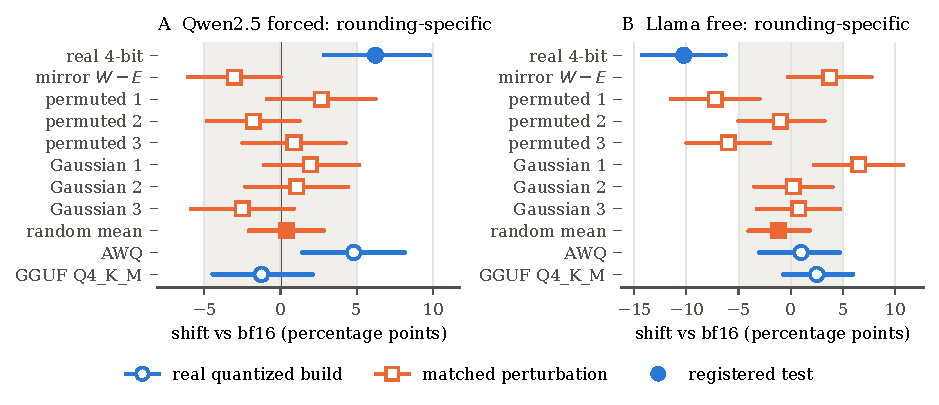
\includegraphics[width=\textwidth]{figures/controls.pdf}
\caption{Every control build in each cell with a shift, as a shift against bf16 with a 95\% interval, beside AWQ and llama.cpp's Q4\_K\_M. Filled markers are confirmatory tests; the panel title gives the verdict of the decision rule in \S\ref{sec:controls}.}
\label{fig:controls}
\end{figure*}

\begin{table*}[t]
\centering\small
% generated by analysis/make_numbers.py -- do not edit
\begin{tabular}{lllrl}
\toprule
Cell & Build & $\Delta$NLL/token & Norm ratio & Shift [95\% CI] \\
\midrule
Qwen2.5 forced & real 4-bit & +0.144 & -- & +6.2 [+2.8, +9.8] \\
 & dense $W+E$ & +0.144 & 1.000 & +4.8 [+1.2, +8.4] \\
 & mirror $W-E$ & +0.131 & 1.000 & $-$3.0 [$-$6.0, +0.0] \\
 & permuted 1 & +0.166 & 1.000 & +2.7 [$-$0.9, +6.2] \\
 & permuted 2 & +0.180 & 1.000 & $-$1.8 [$-$4.8, +1.2] \\
 & permuted 3 & +0.155 & 1.000 & +0.9 [$-$2.5, +4.3] \\
 & Gaussian 1 & +0.168 & 1.000 & +2.0 [$-$1.1, +5.2] \\
 & Gaussian 2 & +0.138 & 1.000 & +1.1 [$-$2.3, +4.4] \\
 & Gaussian 3 & +0.178 & 1.000 & $-$2.5 [$-$5.9, +0.9] \\
 & $W+\tfrac12E$ & +0.033 & 0.500 & +2.7 [$-$0.5, +5.9] \\
 & $W+2E$ & +0.855 & 2.000 & +10.7 [+6.4, +14.9] \\
\addlinespace
Llama free & real 4-bit & +0.038 & -- & $-$10.3 [$-$14.2, $-$6.2] \\
 & dense $W+E$ & +0.038 & 1.000 & $-$10.7 [$-$14.8, $-$7.0] \\
 & mirror $W-E$ & +0.061 & 1.000 & +3.7 [$-$0.2, +7.8] \\
 & permuted 1 & +0.067 & 1.000 & $-$7.3 [$-$11.5, $-$3.0] \\
 & permuted 2 & +0.066 & 1.000 & $-$1.0 [$-$5.0, +3.2] \\
 & permuted 3 & +0.069 & 1.000 & $-$6.0 [$-$10.0, $-$2.0] \\
 & Gaussian 1 & +0.067 & 1.000 & +6.5 [+2.2, +10.8] \\
 & Gaussian 2 & +0.065 & 1.000 & +0.3 [$-$3.5, +4.0] \\
 & Gaussian 3 & +0.061 & 1.000 & +0.8 [$-$3.2, +4.8] \\
 & $W+\tfrac12E$ & +0.005 & 0.500 & $-$5.8 [$-$9.2, $-$2.2] \\
 & $W+2E$ & +0.224 & 2.000 & $-$17.8 [$-$22.5, $-$12.8] \\
\bottomrule
\end{tabular}

\caption{Matched-perturbation builds. $\Delta$NLL is against bf16 on bf16's own harmless replies; the norm ratio is the realized perturbation norm over $\lVert E\rVert$, identical across matrices to the precision shown.}
\label{tab:controls}
\end{table*}

\paragraph{Error structure of the quantizers.} Table~\ref{tab:errors} compares the quantizers' errors with the default round-to-nearest (RTN) error, matrix by matrix over the \N{err.qwen.nmat} (\qwen) and \N{err.llama.nmat} (\llama) quantized matrices. GPTQ's error is the closest to RTN's in direction (median cosine \N{err.qwen.cosrtngptq} and \N{err.llama.cosrtngptq}); MXFP4's is nearly orthogonal to it. AWQ rescales input channels and folds the scales into adjacent layers, so its weights are not directly comparable with $W$ and we report only the cosine.

\begin{table*}[t]
\centering\small
% generated by analysis/make_numbers.py -- do not edit
\begin{tabular}{lrrrrrr}
\toprule
 & \multicolumn{3}{c}{median relative error} & \multicolumn{3}{c}{median cosine with RTN error} \\
\cmidrule(lr){2-4}\cmidrule(lr){5-7}
Model & RTN & MXFP4 & GPTQ & MXFP4 & GPTQ & AWQ \\
\midrule
\qwen & 0.094 & 0.118 & 0.115 & 0.11 & 0.31 & 0.04 \\
\llama & 0.093 & 0.118 & 0.111 & 0.07 & 0.32 & 0.13 \\
\bottomrule
\end{tabular}

\caption{Per-matrix error of each quantizer: relative error $\lVert \hat W - W\rVert / \lVert W\rVert$, and cosine between its error and the RTN error.}
\label{tab:errors}
\end{table*}

\section{Free-start development set}
\label{app:pilot}
The first 200 WildJailbreak prompts form the development set (Table~\ref{tab:pilot}); the free-start test uses the 400 held-out prompts. \llama's 4-bit build was \N{pilot.llama.4bit-g64.diff}\pp{} against bf16 and \qwenthree's \N{pilot.qwenthree.4bit-g64.diff}\pp. On the held-out prompts the first holds and the second does not (\S\ref{sec:free}).

\begin{table*}[t]
\centering\small
% generated by analysis/make_numbers.py -- do not edit
\begin{tabular}{llrrlrll}
\toprule
Model & Build & bf16 \% & build \% & Shift [95\% CI] & Disc. & $p$ & Holm $p$ \\
\midrule
\qwen & 4-bit & 48.5 & 53.5 & +5.0 [$-$1.5, +11.5] & 19/29 & $0.19$ & -- \\
\qwen & MXFP4 & 48.5 & 49.5 & +1.0 [$-$6.0, +8.0] & 25/27 & $0.89$ & -- \\
\llama & 4-bit & 45.0 & 30.5 & $-$14.5 [$-$20.5, $-$8.5] & 34/5 & $2.4\times10^{-6}$ & -- \\
\llama & MXFP4 & 45.0 & 34.0 & $-$11.0 [$-$17.0, $-$5.0] & 31/9 & $6.8\times10^{-4}$ & -- \\
\qwenthree & 4-bit & 23.5 & 33.5 & +10.0 [+5.0, +15.0] & 4/24 & $1.8\times10^{-4}$ & -- \\
\qwenthree & MXFP4 & 23.5 & 23.0 & $-$0.5 [$-$5.0, +4.0] & 11/10 & $1.00$ & -- \\
\bottomrule
\end{tabular}

\caption{Free-start development set, 200 prompts. No correction is applied.}
\label{tab:pilot}
\end{table*}

\section{End-of-turn failure in MXFP4 \qwen}
\label{app:runon}
MXFP4 \qwen{} sometimes fails to end its turn and writes a fabricated next user turn. On 200 benign prompts with a 512-token cap this happens in \N{s5.qwen.mxfp4}\% of replies and in no other build we tested (Table~\ref{tab:runon}). It persists when the weights are dequantized to bf16 (\N{s5.qwen.mxfp4dequant}\%), so it comes from the weights and not from the kernel, and it does not appear in MXFP4 Qwen2.5-0.5B.

\begin{table*}[t]
\centering\small
% generated by analysis/make_numbers.py -- do not edit
\begin{tabular}{lrrrrrrr}
\toprule
Model & bf16 & 8-bit & 4-bit g32 & mixed 4/6 & 4-bit & MXFP4 & MXFP4 deq. \\
\midrule
\qwen & 0.0 & 0.0 & 0.0 & 0.0 & 0.0 & 10.5 & 8.5 \\
\llama & 0.0 & -- & -- & -- & 0.0 & 0.0 & -- \\
\qwenthree & 0.0 & -- & -- & -- & 0.0 & 0.0 & -- \\
Qwen2.5-0.5B & 0.0 & -- & -- & -- & 0.0 & 0.0 & 0.0 \\
\bottomrule
\end{tabular}

\caption{Share (\%) of replies to 200 benign prompts that contain a fabricated next turn (512-token cap). ``--'': not built for that model.}
\label{tab:runon}
\end{table*}

\section{Compute, software and release}
\label{app:compute}
All runs used one Apple M2 Pro with 16\,GB of memory, \texttt{mlx} 0.32.4 and \texttt{mlx-lm} 0.32.2, with one model in memory at a time. The logged experiment runs took about \N{compute.hours} hours over \N{compute.steps} steps, building, generating and judging; this excludes development. The bf16 checkpoints are identified by the first twelve hex digits of the SHA-256 over their weight files: \qwen{} \texttt{\N{hash.qwen}}, \llama{} \texttt{\N{hash.llama}}, \qwenthree{} \texttt{\N{hash.qwenthree}}.

We release the code, the pre-registration, the prompt identifiers, every judge and human label, the perturbation builder and the analysis that produces every number in this paper. We do not release the replies themselves, which include harmful content produced under a forced start; they are available to researchers on request.

\paragraph{Use of AI assistants.} AI assistants were used for coding, literature search and editing of the text. The author takes full responsibility for the content.
